\chapter{Contributions}
\label{chap:contributions}

As we will see in the Experiments, the local Bayesian optimization technique is more efficient than the commonly used global one. We implement this local Bayesian algorithm developed by \cite{akrour2017local} and we also contribute a trajectory kernel suited for the Thompson sampling acquisition function used by the proposed algorithm.

\section{Local Bayesian optimization}
\label{sec:localBO}
Modelling the objective function for a higher dimensional search space is challenging. Also global Bayesian optimization tends to over-explore. To perform a more robust optimization we use local Bayesian optimization as stated in \cite{akrour2017local}. It restricts the search space of the acquisition function to a local area which is moved, resized, and rotated between iterations. This local area is defined by a Gaussian distribution in which the mean and variance represent the centre and the exploration reach respectively. To update that mean and variance properly we minimize the Kullback-Leibler divergence between the current search distribution $\pi_n$ and the probability $p_n^* = p(\x=\x^*|\mathcal{D}_n)$ of $\x^*$ being optimal. This results in a search area which neglects poorly performing regions.

To prevent the mean from moving too fast from the initial point and to avoid the variance becoming too small quickly the minimization is constrained with the hyper parameters $\alpha$ and $\beta$. Therefore our optimization problem is given by

\begin{align}
    & \underset{\pi}{\arg\min} & & \KL(\pi||p_n^\star),& &\notag\\
    & \text{subject to}
    & & \KL(\pi||\pi_n) & &\leq \alpha,\label{eq:kl:our}\\
    & & &\HH(\pi_n) - \HH(\pi) & &\leq \beta,\label{eq:entropy:our}
\end{align}

where $\KL(.||.)$ denotes the Kullback-Leibler divergence $\mathcal{H}(p) = -\int p(\x)\log(p(\x)) d\x$ is the entropy of $p$. We implement the local Bayesian optimization as suggested in \cite{akrour2017local}.

% \begin{algorithm}[t]
%    \caption{Local Bayesian Optimization\label{alg:localBO}}
%    \SetKwInOut{Input}{input}\SetKwInOut{Output}{output}
%
%    \Input{Initial search policy $\pi_0 = \mathcal{N}(\boldsymbol{\mathrm{m}}_0, \sigma_0^2I)$\\ step-size $\epsilon$\\ entropy reduction rate $\beta$}
%    \Output{Search policy $\pi_N$}
%    \BlankLine
%    \For{$n=1$ \KwTo $N$}{
%        \textit{{\small Fit:}} Gaussian $\pntilde$ from local samples of $\pnstar$ \hfill\\
%        \textit{{\small Optimize:}} $(\eta^*, \omega^*) = \arg\min g_n(\eta, \omega)$ \hfill\\
%     %   \STATE  Compute weights $\gstar = \frac{\estar}{\estar + \ostar}$ and $\lstar = \frac{1}{\estar + \ostar}$
%        \textit{{\small Bayesian Update:}} $\left(\pi_{n+1}\right)^{\estar + \ostar}  \propto \pi_{n}^{\estar} \pnstar$ \hfill\\
%        \textit{{\small Evaluate:}} $\x_n$ from local samples of $\pnstar$ \hfill \\
%        $\Data_n   \longleftarrow \Data_{n-1} \cup \{(\x_n, y_n)\}$
%    }
% \end{algorithm}


\subsection{Constraint Thompson sampling}

To perform Thompson sampling on the variable search distribution we first sample a number of points from the current search distribution (algorithm \ref{alg:acqLocalBO}). Then we compute the Mahalanobis distance for each test point to discard samples, which are at the outer edge of the search space. The Mahalanobis distance is used to regard the covariance of the current search distribution in distance computations.

\begin{algorithm}
    \caption{Thompson sampling acquisition for local Bayesian optimization\label{alg:acqLocalBO}}
    \SetKwInOut{Input}{input}\SetKwInOut{Output}{output}
    \Input{$X$ = $n$ already evaluated points\\$X_*$ = random samples from the search distribution\\$d_t$ = distance threshold}
    \Output{$\mathbf{x}_{n+1}$: next evaluation point}
    \BlankLine

    compute the Mahalanobis distance from test points to current search distribution\\
    keep samples, which are inside the distance threshold $d_t$ of the distribution density\\
    get mean and covariance matrix from the Gaussian process\\
    get values from Thompson sampling\\
    $\mathbf{x}_{n+1}$ = sample at the maximum of Thompson sampled values\\
\end{algorithm}

\subsection{Trajectory kernel for local Bayesian optimization}
\label{sec:ownTK}
If using Thompson sampling as the acquisition function, the whole covariance matrix $V$ of test points is needed. To compute this covariance matrix, we need a distance measure between unknown trajectories. The kernel proposed by \cite{wilson2014using} does not support a measurement between unevaluated policies. We therefore implement our own distance metric based on states, which are already present in the training data. First we filter a random subset from the training data and save it to $S_{\text{sub}}$. For the continuous action space we then calculate each mean
$$m_i = f_s(S_{\text{sub}})^\top \mathbf{x}_i \qquad \text{and}\qquad m_j = f_s(S_{\text{sub}})^\top \mathbf{x}_j$$
for the given policies $\mathbf{x}_i$ and $\mathbf{x}_j$. The difference between the two policies is measured by the squared Euclidean distance between the means:
$$D(\mathbf{x}_i,\mathbf{x}_j) = (m_i - m_j)^\top (m_i - m_j).$$
For the discrete action space we sample the actions $\mathbf{a}$ from $p(\mathbf{a}|S_{\text{sub}},x)$ for the given policies $\mathbf{x}_i$ and $\mathbf{x}_j$ from (\ref{eq:discreteactionselection}). The sampled actions then select the associated probability values. We compare the sets of probability values for each policy by applying the discrete Kullback-Leibler divergence
$$D(\mathbf{x}_i,\mathbf{x}_j) = \sum p(\mathbf{a}_i)\,\log {\frac {p(\mathbf{a}_i)}{p(\mathbf{a}_j)}} + \sum p(\mathbf{a}_j)\,\log {\frac {p(\mathbf{a}_j)}{p(\mathbf{a}_i)}},$$

where $\mathbf{a}_i$ denotes the actions sampled from the probabilities $p(\mathbf{a}|S_{\text{sub}},\mathbf{x}_i)$ and $p(\mathbf{a}_i)$ the corresponding probabilities. As in the other trajektory kernel (section \ref{sec:trajKernel}) we add the both Kullback-Leibler divergences to get a symmetric distance measure.

% \begin{algorithm}
%     \caption{Thompson Sampling acquisition for Local Bayesian optimization\label{alg:acqLocalBO}}
%     \SetKwInOut{Input}{input}\SetKwInOut{Output}{output}
%     \Input{$X$: $N$ already evaluated points\\$X_*$: $M$ random samples from the search distribution}
%     \Output{$x_{n+1}$: next evaluation point}
%     \BlankLine
%
%     $m_d$ = Mahalanobis distance from test points to incumbent search distribution\\
%     discard samples, which are outside $80\%$ of the cumulative inverse-chi-squared distribution\\
%     get mean and covariance matrix from the Gaussian process\\
%     get values from Thompson sampling\\
%     $x_{n+1}$ = sample at the highest Thompson sampled value\\
% \end{algorithm}

\section{Numerical stability and efficiency}
Due to numerical instabilities, errors may occur during calculations. These errors are caused by the discrete implementation of continuous mathematical formulas. Sometimes numerical instabilities lead to negative values for covariances. To avoid getting complex numbers we assume negative values as zero before applying the square root on covariances when computing the standard deviation from the Gaussian process model (\ref{eq:gp:stdv}). Negative values can also occur for the distance between two trajectories, and are thresholded to zero, too.\\

When computing the symmetrical distance matrix $\hat{D}(X,X)$ (\ref{eq:tk:mc}) only the upper triangle matrix $\hat{D}_{u}$ is calculated. That halves the computational effort. We obtain $\hat{D} = \hat{D}_{u}+\hat{D}_{u}^\top$, since the diagonal elements of $\hat{D}$ are zero and $\hat{D}(\mathbf{x}_i,\mathbf{x}_j) = \hat{D}(\mathbf{x}_j,\mathbf{x}_i)$.\\

To gain robustness we use the lower Cholesky decomposition instead doing matrix inverse calculation. Therefore, the matrix to decompose must be positive definite. We achieve this by doubling the noise variance added to the diagonal elements of the original matrix as shown in algorithm \ref{alg:cholesky}.

\begin{algorithm}
    \caption{Lower Cholesky with variance doubling\label{alg:cholesky}}
    \SetKwInOut{Input}{input}\SetKwInOut{Output}{output}
    \Input{$K$, $\sigma_n$}
    \Output{$L$}
    \BlankLine
    $K_n = K+\sigma_n^2 I$\\
    \While{$K_n$ not positive definite}{
        double $\sigma_n^2$\\
        $K_n = K+\sigma_n^2 I$\\
    }
    $L$ = lower Cholesky of $K_n$\\
\end{algorithm}

When doing hyper parameter optimization, we do not double the noise variance. Instead our log marginal likelihood function (\ref{eq:hypOpt}) returns negative infinity for hyper parameters, which produce a non positive definite matrix $K_n$. Therefore, such hyper parameters do not come into consideration when maximizing.

\subsection{Gaussian process regression}

Since the prior covariance matrix $K_n$ (and therefore its Cholesky decomposite $L$) does not change during the acquisition function optimization it can be pre-computed to make the Gaussian process regression more efficient. Additionally we customize the computation of the variance vector to lower the computational effort.

\subsubsection{Inverse of prior covariance matrix}

Instead of calculating the inverse of $K_n$ in \eqref{eq:meanGauss} we use the Cholesky decomposed matrix:

$$LL^\top=K_n$$

This is considered faster and numerically more stable \cite{rasmussen2006gaussian}. The mean vector $\mathrm{m}$ is then computed as follows:

\begin{equation} \label{eq:regression}
    \mathbf{m} = K_n^{-1}\,y = (L\,L^{\top})^{-1}\,\mathbf{y} = (L^{-\top}\,L^{-1})\,\mathbf{y} = L^{-\top}\,(L^{-1}\,\mathbf{y}) = L^{\top}\setminus(L \setminus \mathbf{y}).
\end{equation}

The backslash operator denotes the matrix left division, so the solution $\mathbf{x}=A\setminus \mathbf{b}$ satisfies the system of linear equations $A\,\mathbf{x}=\mathbf{b}$.
Matrix $K_n$ must be positive definite for the Cholesky decomposition. So we double the noise variance hyper parameter $\sigma_n^2$ as shown in algorithm \ref{alg:cholesky}.

\subsubsection{Variances}

For the expected improvement function, we only need the vector of variances. Instead of calculating the whole covariance matrix $V$ and taking the diagonal elements (\ref{eq:vectorVar}) we can take a shortcut. All elements on the diagonal of $K(X_*,X_*)$ equal $\sigma_f^2$ because the difference between one $\mathbf{x}_*$ and the same $\mathbf{x}_*$ is zero. Therefore we can write:

\begin{align}
    L_k &= L \setminus K(X_*,X) \\
    v &= \sigma_f - \sum_{\text{rows}} (L_k \circ L_k). \label{eq:vectorvar}
\end{align}

This adaptation is inspired by \cite{nandoCode} and reduces the computational effort drastically from $\mathcal{O}(n^2)$ to $\mathcal{O}(n)$.

For the whole covariance matrix for Thompson sampling we also avoid calculating the matrix inverse:

$$V = K(X_*,X_*) - (L_k^\top L_k)^\top $$

\subsection{Action selection}

In continuous action space our stochastic policy is Gaussian distributed (\ref{eq:actionselection}). Therefore the resulting probability density of the action selection,

$$P_{\pi}(\mathbf{a}|\mathbf{s},\mathbf{x}) = \frac{1}{\sqrt{2\pi\sigma_a^2}}\exp\left(-\frac{(\mathbf{a}-f_s(\mathbf{s})x)^2}{2\sigma_a^2}\right),$$

allows us to do the computations of the logarithm of the probability ratios in the trajectory kernel more efficient:

\begin{align*}
    \sum_{t=1}^{t_\mathrm{max}} \log \left(\frac{P_{\pi}(a_{t}|s_{t},\mathbf{x}_i)}{P_{\pi}(a_{t}|s_{t},\mathbf{x}_j)}\right) &= \sum_{t=1}^{t_\mathrm{max}} \log \left(\frac{\frac{1}{\sqrt{2\pi\sigma_a^2}}\exp\left(-\frac{(a_t-f_s(\mathbf{s}_t)\mathbf{x}_i)^2}{2\sigma_a^2}\right)}{\frac{1}{\sqrt{2\pi\sigma_a^2}}\exp\left(-\frac{(a_t-f_s(\mathbf{s}_t)\mathbf{x}_j)^2}{2\sigma_a^2}\right)}\right)\\
    &= \sum_{t=1}^{t_\mathrm{max}} \log \left( \exp \left( -\frac{(a_t-f_s(\mathbf{s}_t)\mathbf{x}_i)^2}{2\sigma_a^2} - \left(-\frac{(a_t-f_s(\mathbf{s}_t)\mathbf{x}_j)^2}{2\sigma_a^2}\right)\right)\right)\\
    &= \frac{1}{2\sigma_a^2} \sum_{t=10}^{t_\mathrm{max}} \left((a_t-f_s(\mathbf{s}_t)\mathbf{x}_j)^2 - (a_t-f_s(\mathbf{s}_t)\mathbf{x}_i)^2\right).
\end{align*}

\subsection{Hyper parameter optimization}

Especially for the trajectory kernel we want a hyper parameter optimization, because all the values of the distance matrix $D$ may get very big. When dividing by a well tuned hyper parameter $\sigma_l$ before applying the exponential function \eqref{eq:trajKernel}, we avoid getting a diagonal matrix $K$ or a zero matrix $K_*$.\\

When calculating $\log(|K_n|)$ for the hyper parameter optimization \eqref{eq:hypOpt}, again we use the Cholesky decomposition of $K$. Thus the determinant transforms to
$$|K_n|=|L\,L^{T}|=|L|\,|L^{T}|=|L|\,|L|=|L|^{2}.$$

Since the determinant of the Cholesky decomposed matrix,
$$|L| = \textstyle\prod_{i} L_{ii},$$
is the product of its diagonal elements, we can transform this into a numerically more stable version:

$$\log(|K_n|) = \log(|L|^{2}) = 2\,\log(|L|) = 2\,\log(\textstyle\prod_{i} L_{ii}) = 2\textstyle\sum_{i} \log(L_{ii}).$$

The computation of $K_y^{-1}\mathbf{y}$ in \eqref{eq:hypOpt} is done by the same method we already use in the Gaussian process \eqref{eq:regression}.

For debugging purposes and for estimating the quality of the hyperparameter optimization, we plotted a grid of values generated by the log marginal likelihood function during development and testing. Figure \ref{fig:hyp} contains a very stable example of the hyper parameter space.

\subsubsection{Independent log-normal prior}
The log marginal likelihood maximization will sometimes succeed at the borders of our search space resulting in very high high or very low hyper parameters. We prevent this by adding an independent log-normal prior term as introduced in \cite{lizotte2008practical}:

$$\sum_{i=f,l}\left(\frac{-\log(\sigma_i)^2}{2\cdot 10^2} - \log\left(10\sqrt{2\pi}\right) \right).$$

Since the suggested prior is centred at the point of origin with standard deviation 10, but we want our search space to adapt between iterations, we make the mean and the standard deviation adjustable. We write:

$$\sum_{i=1,2}\left(\frac{-(h_i-c_i)^2}{2(b_{u_i}-b_{l_i})^2} - \log\left((b_{u_i}-b_{l_i})\sqrt{2\pi}\right) \right),$$

where $b_l$ and $b_u$ denote the lower and upper bounds of the search space and $c$ its center. And since we optimize over the logarithmic space $h_1 = \log\sigma_f$ and $h_2 = \log\sigma_l$.

\begin{figure}[H]
    \centering
    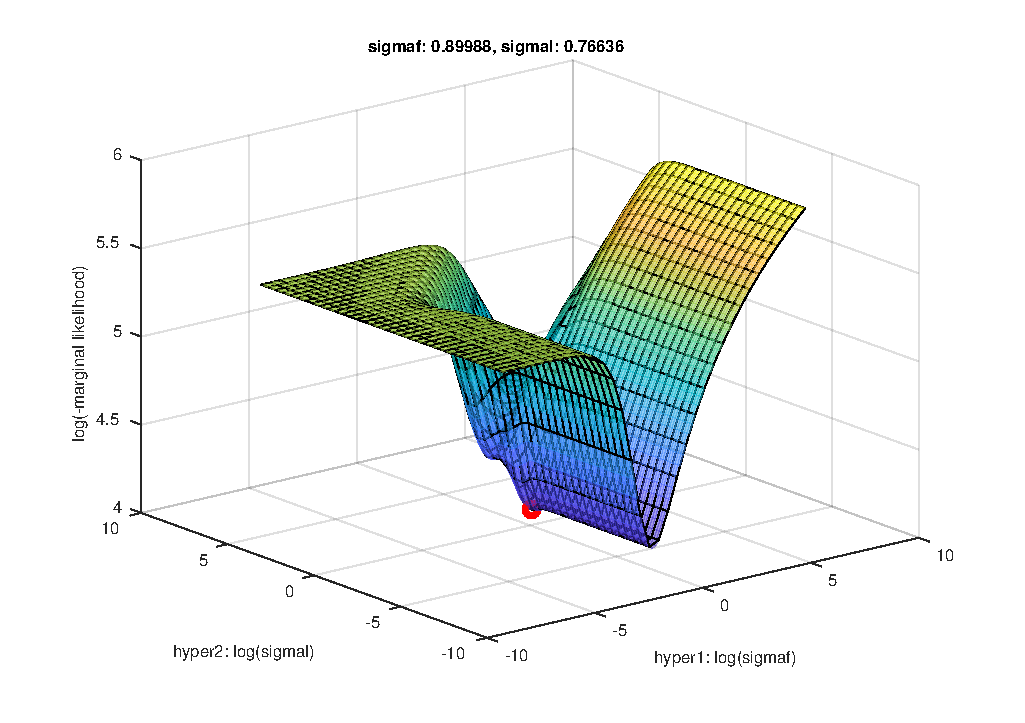
\includegraphics{/home/sebastian/Documents/bscThesis/img/hyper.pdf}
    \caption{Exemplary hyper parameter minimization plot with the optimum marked as the red circle.\label{fig:hyp}}
\end{figure}
